Using feedback from the force-torque sensors the Hubo-Ach controller adds compliance to the legs via active damping.
Fig.~\ref{fig:activedamping} shows as the user pushes down on the robot the force is detected by the force-torque (FT) sensors.
This then modifies the joint commands such that the center of mass (CoM) acts like there is an over-damped spring-damper system between it and mechanical ground.

\begin{figure}[thpb]
  \centering
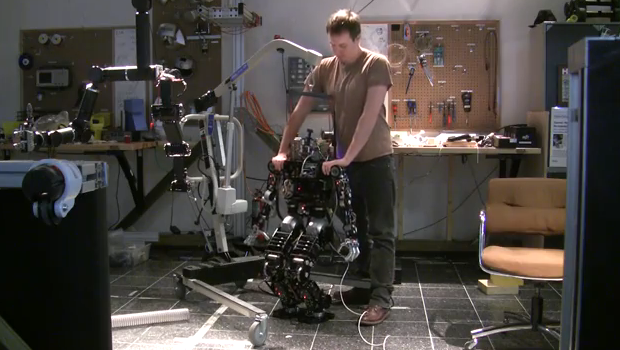
\includegraphics[width=0.6\columnwidth]{./pix/activedamping.png}

\includegraphics[width=0.3\columnwidth]{./qrcode/qrcode-activedamping.png}\\
     http://danlofaro.com/phd/tracking/\#TrackingAndWalking
  \caption{Using feedback from the force-torque sensors the Hubo-Ach controller adds compliance to the legs via active damping. }
  \label{fig:activedamping}
\end{figure}
